\chapter{Benutzerhandbuch\label{appendix_A}}

%!TEX root=../Benutzerhandbuch.tex
\chapter{Einleitung}
Im Verlauf des Maturaprojekts des 5. Jahrgangs der Abteilung IT am TGM wurde von dem Projektteam Peer Nagy, Gabriel Pawlowsky und Josef Sochovsky unter der Betreuung von Prof. Mag. Hans Brabenetz und Dr. Helmut Vana eine Software geschrieben. Der Sinn und Zweck dieser Software ist das Testen eines Algorithmus �ber eine Menge an gegebenen Daten. Ein solcher Algorithmus ist eine automatisierte Entscheidungslogik, die anhand von historischen Aktiendaten Entscheidungen generieren kann. Eine Entscheidung kann eine Kauf- oder Verkaufsentscheidung. \\
Die Software zeigt Qualit�tsmerkmale des Algorithmus �ber die gegebenen Daten an und simuliert somit einen B�rsenablauf.

%!TEX root=../Benutzerhandbuch.tex
\chapter{Installation}
\section{Start der Installation}
Die Installation wird durch das ausführen der setup.exe gestartet. Danach öffnet sich der Installer.
\begin{figure}[H]
\centering
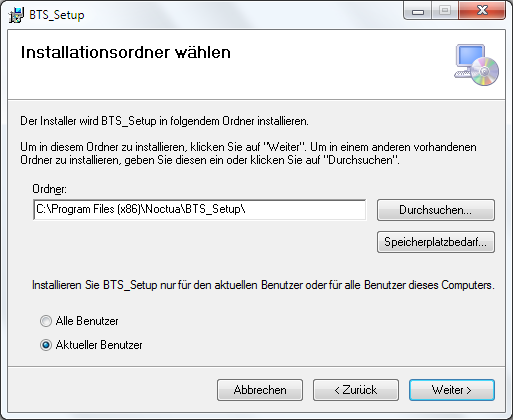
\includegraphics[width=1\textwidth]{images/btsinstall1.png}
\caption{Konfigurieren der Installtion}
\end{figure}
Nach der korrekten Konfiguration des Setups kann die Installtion gestartet werden.
\begin{figure}[H]
\centering
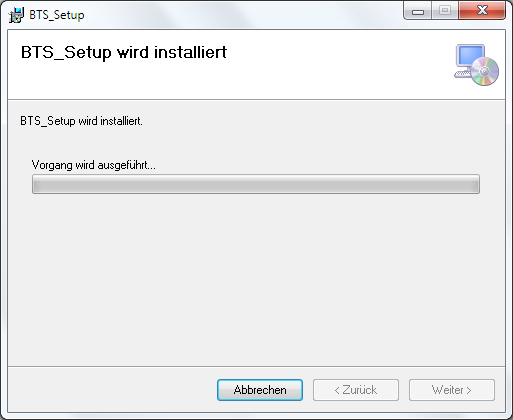
\includegraphics[width=1\textwidth]{images/btsinstall2.png}
\caption{Installationsvorgang}
\end{figure}
Nach diesem Vorgang ist die Backtesting-Software vollständig installiert und ausführbar.
%!TEX root=../Benutzerhandbuch.tex
\section{Programm}
%!TEX root=../../Benutzerhandbuch.tex
\section{Schreiben eines Algorithmus}
Um die Software zu bedienen wird ein in \gls{F-Sharp} geschriebener Algorithmus benötigt. Dieser muss als \gls{DLL}-Datei zur Laufzeit in die Software eingebunden werden. Eine solche Datei wird mittels Microsoft Visual Studio erzeugt werden, damit die Software funktionieren soll. \\
Folgende Eigenschaften muss die Datei erfüllen:
\begin{itemize}
	\item Name der Methode: startCalculation
	\item Übergabeparameter 1: eine Liste aller historischen Daten 
	\item Übergabeparameter 2: eine Liste der Signale für die Entscheidungen (bei Übergabe ist diese Liste leer)
\end{itemize}
Mit dem Rückgabewert der Methode wird nicht gearbeitet, sondern mit der vom Algorithmus verarbeiteten Signalliste.

\begin{lstlisting}[caption=Dateityp des 1. Übergabeparameters]{prices}
System.Collections.Generic.List<System.Tuple
<System.DateTime,decimal,decimal,decimal,decimal>>
\end{lstlisting}
\begin{lstlisting}[caption=Dateityp des 2. Übergabeparameters]{signals}
System.Collections.Generic.List<int>
\end{lstlisting}
Außerdem muss sich der Algorithmus im Namespace  "`Algorithm"' und im Modul "`DecisionCalculator"' befinden.
\subsection{Erzeugen eines Algorithmus-Files}
Öffnen Sie Microsoft Visual Studio und erzeugen sie ein neues Projekt.\\
\begin{figure}[H]
\centering
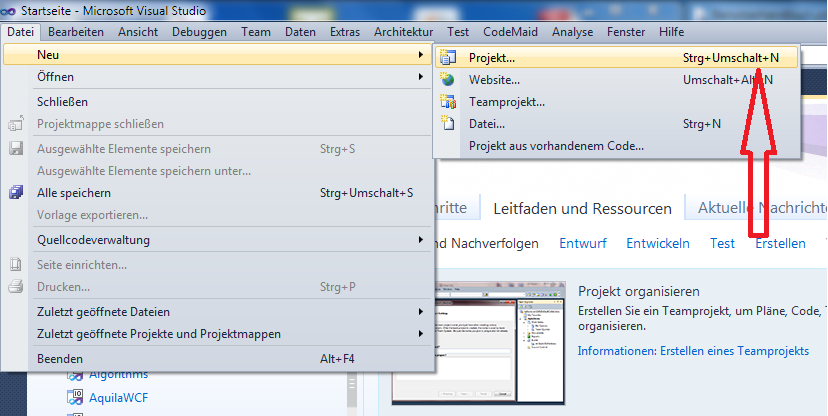
\includegraphics[width=1\textwidth]{images/newProject.png}
\caption{Erzeugen eines neuen Projekts}
\end{figure} 
\newpage
Erstellen Sie es als \gls{F-Sharp}-Bibliothek.
\begin{figure}[H]
\centering
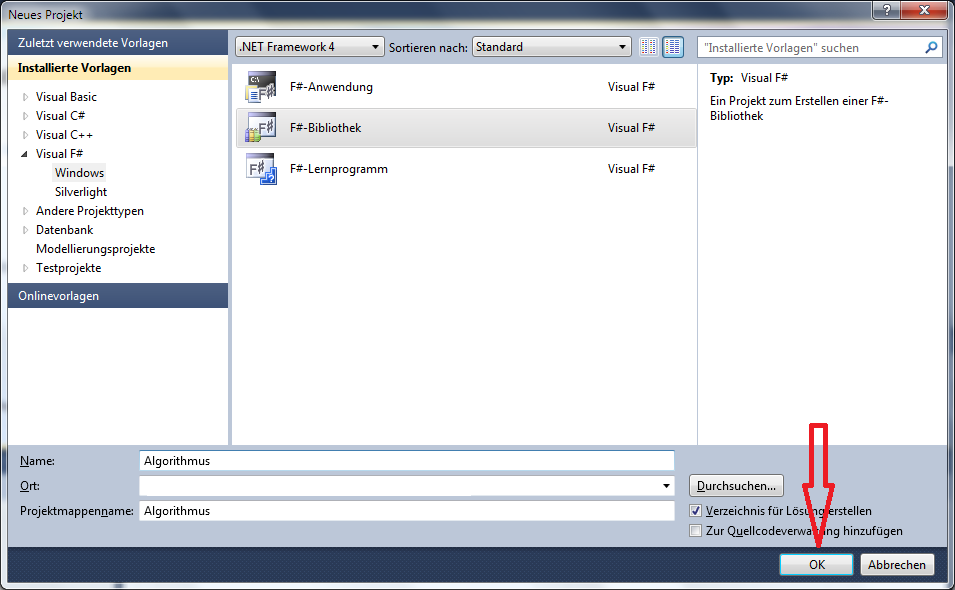
\includegraphics[width=1\textwidth]{images/createProject.png}
\caption{Erstellen Sie es als \gls{F-Sharp}-Bibliothek}
\end{figure}
Halten Sie sich an die, im Kapitel "`Schreiben eines Algorithmus"', genannten Richtlinien und implementieren die Methode startCalculation und kompilieren sie das Projekt.
\begin{figure}[H]
\centering
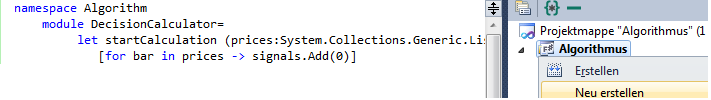
\includegraphics[width=1\textwidth]{images/makeFs.png}
\caption{Kompilieren des Projekts}
\end{figure}
\clearpage
\subsection{Entscheidungen}
Folgende Entscheidungen sind zulässig:
\begin{center}
\begin{tabular}{ |  p{1cm} | p{8cm} |}
\hline 
3 & starkes Kaufssignal \\ \hline
2 &   mittleres Kaufssignal \\ \hline
1 &  schwaches Kaufssignal\\ \hline
0 &  Alle Bestände werden gekauft oder verkauft\\ \hline
-1 &  schwaches Verkaufssignal\\ \hline
-2 &  mittleres Verkaufssignal\\ \hline
-3 &  starkes Verkaufssignal\\ \hline
\end{tabular}
\end{center}

%!TEX root=../../Benutzerhandbuch.tex
\section{Historische Daten}

Um einen Algorithmus mit der \gls{BTS} testen zu k�nnen, m�ssen auch noch historische Aktien-Preisdaten in die Software eingebunden werden, �ber die der Algorithmus getestet wird. Diese k�nnen in Form einer \gls{CSV}-Datei gespeichert und ihr Pfad in der \gls{BTS} angegeben werden. Dabei wurde ein sehr weit verbreitetes Format benutzt, das bspw. auch jegliche Software des renomierten Aktiendatenbereitstellungs-Unternehmens eSignal exportieren kann. Au�erdem werden in dieser Datei die historischen Daten in Form von \glspl{Bar} �ber einen bestimmten Zeitraum (z.B. Daily-\gls{Bar} oder Minute-\gls{Bar}) erwartet und nicht als einzelne Preiswerte. Das Format sieht in etwa so aus:

\begin{lstlisting}[caption=Aufbau der \gls{CSV}-Datei]{csv}
Bar,Date,Time,Open,High,Low,Close
1,01/02/90,00:00,8.8125,9.375, 8.75,9.3125
2,01/03/90,00:00,9.375, 9.50,9.375,9.375
3,01/04/90,00:00,9.375,9.6875,9.3125,9.40625
...
\end{lstlisting}

Zuerst steht also die Nummer des Bars, die allerdings nicht ber�cksichtigt wird. Darauf folgt das Datum in der Form \inline{MM/DD/YY} und die Uhrzeit in der Form \inline{hh:mm}. Zu guter Letzt kommen nun nur noch die Werte Open, High, Low und Close des \glspl{Bar}. Diese Datei kann nahezu unendlich lange gemacht werden, es k�nnen also nahezu unendlich viele Bars nach unten hin erg�nzt werden. Die erste Zeile der Datei wird im Allgemeinen nicht ber�cksichtigt, da sie meist die �berschriften enth�lt. Sollte sich in der ersten Zeile also ein Bar befinden, wird dieser ebenfalls ignoriert.
%!TEX root=../../Benutzerhandbuch.tex
\section{Backtestingsoftware}

Die \gls{BTS} ist nun also die Kernsoftware, mit der die Algorithmen �ber Daten-Files getestet werden k�nnen. Dazu sollten zuerst die allgemeinen Einstellungen get�tigt werden. Diese befinden sich im Settings-Tab unter ''Orders'' und sehen so aus:

\begin{figure}[H]
\centering
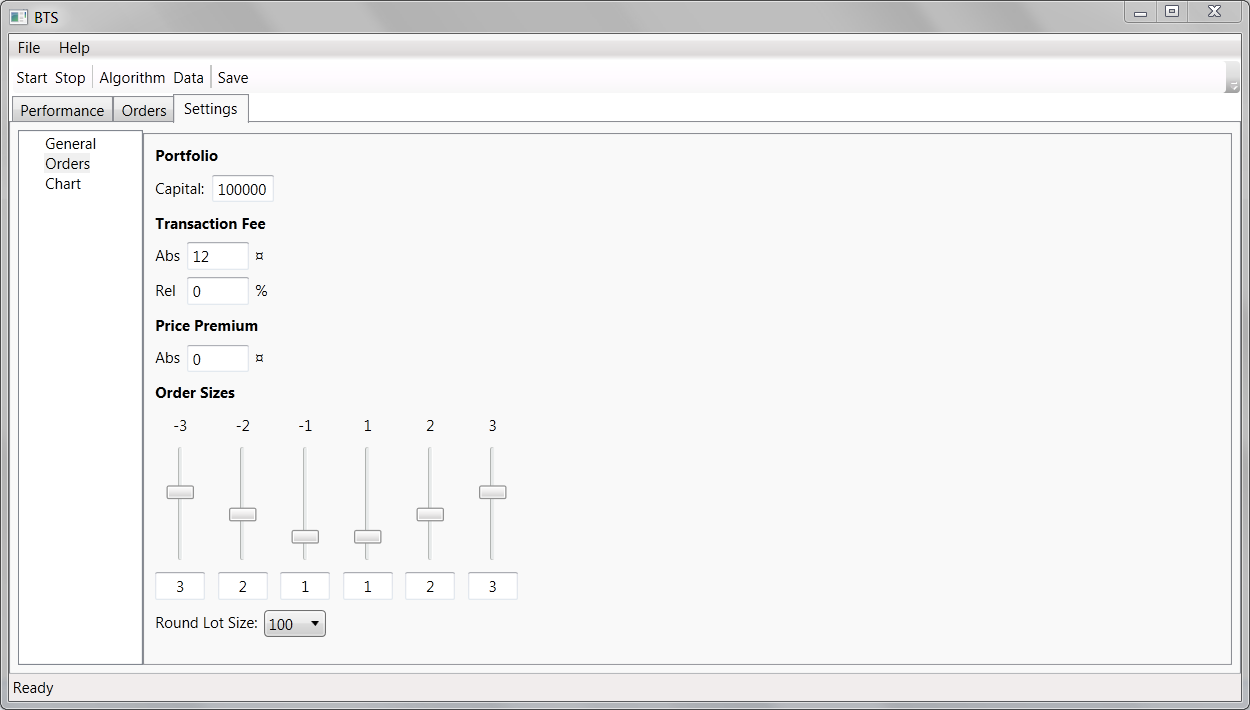
\includegraphics[width=1\textwidth]{images/btsordersettings.png}
\caption{Order-Settings der \gls{BTS}}
\end{figure}

Hier kann zuerst das gew�nschte Kapital eingestellt werden, dessen Handel die \gls{BTS} simulieren soll. Danach k�nnen Transaktionsgeb�hren absolut oder relativ, ein Preisaufschlag f�r K�ufe und die Order-Gr��en eingestellt werden. Die Order-Gr��en geben an, wie viele Round Lots bei einem Signal von -3 bis +3 gekauft/verkauft werden sollen. Ein Round Lot ist hierbei die kleinste �ber einen Online-Broker erwerbbare Menge an Aktien, die ebenfalls variieren und daher eingestellt werden kann.\\ \\

Auf der Seite darunter, der ''Chart''-Seite, k�nnen verschiedene Indikatoren aus der Combobox ausgew�hlt und hinzugef�gt werden, die dann nach der Performancemessung in die Grafik im Orders-Tab eingezeichnet werden. Hier k�nnen au�erdem f�r jeden Indikator die entsprechend notwendigen Parameter und Farben ausgew�hlt werden.

\begin{figure}[H]
\centering
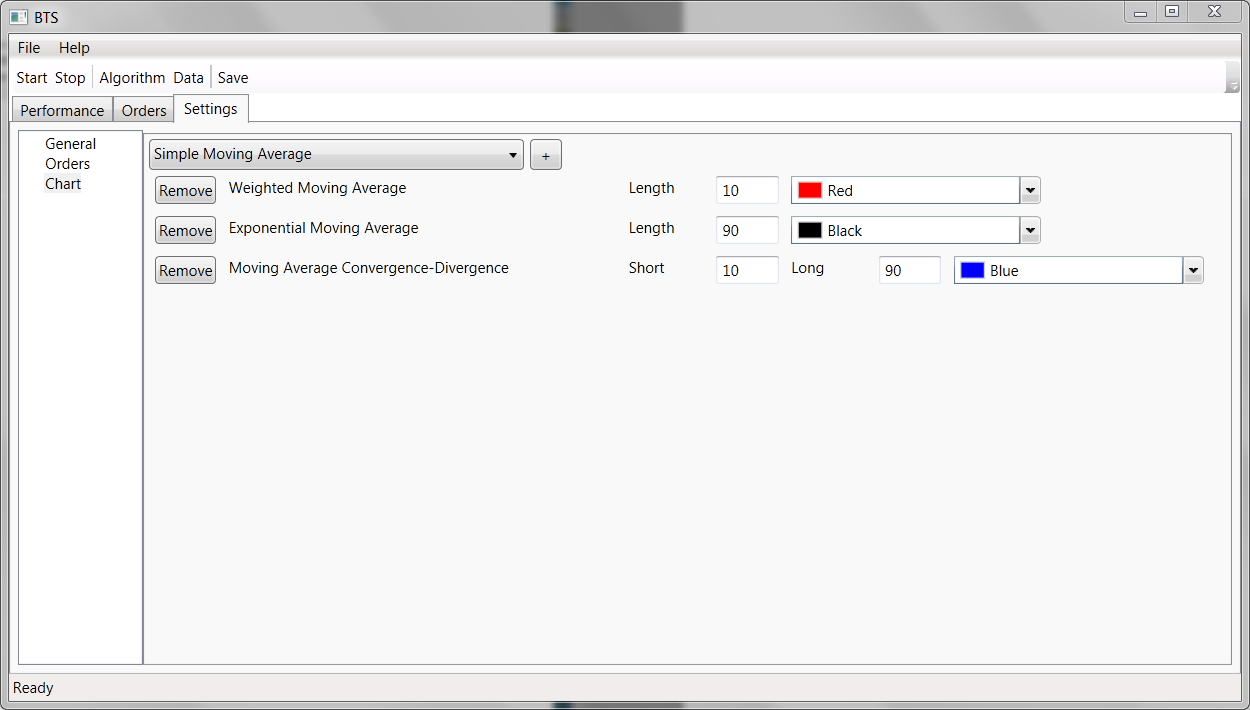
\includegraphics[width=1\textwidth]{images/btschartsettings.png}
\caption{Chart-Settings der \gls{BTS}}
\end{figure}

Weiters k�nnen nun unter der Seite ''General'' die eigentlich wichtigsten Informationen festgelegt werden. Diese sind die Pfade zur Algorithmus- und zur Daten-Datei, die in den vorherigen Punkten erl�utert wurden. Diese Pfade k�nnen �brigens auch durch den ''Algorithm''- und den ''Data''-Button in der Men�leiste hinzugef�gt werden. Darunter kann noch eine Zeitspanne ausgew�hlt werden. Der Algorithmus wird dann nur �ber alle Daten getestet, die im Daten-File im gew�hlten Zeitraum vorkommen.

\begin{figure}[H]
\centering
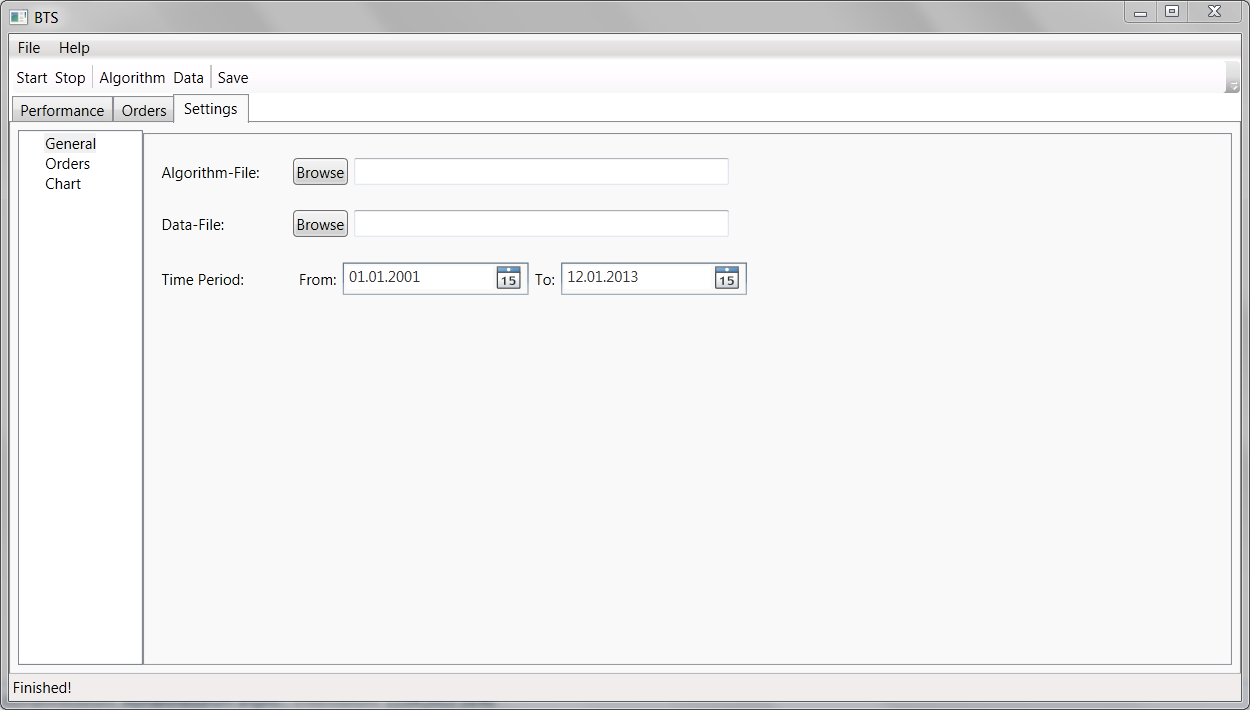
\includegraphics[width=1\textwidth]{images/btsgeneralsettings.png}
\caption{General-Settings der \gls{BTS}}
\end{figure}

Nachdem alle Einstellungen getroffen wurden, kann der Test gestartet werden.

\begin{figure}[H]
\centering
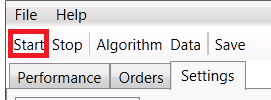
\includegraphics[width=0.6\textwidth]{images/btsstart.png}
\caption{Start-Button der \gls{BTS}}
\end{figure}

Anschlie�end werden auf dem Performance-Tab der \gls{BTS} die allgemeinen Performance-Daten des Algorithmus �ber das spezifizierte Daten-File ausgegeben. N�here Erkl�rungen zu diesen Werten k�nnen durch Halten der Maus �ber einen der Texte als Tooltip angezeigt werden.

\begin{figure}[H]
\centering
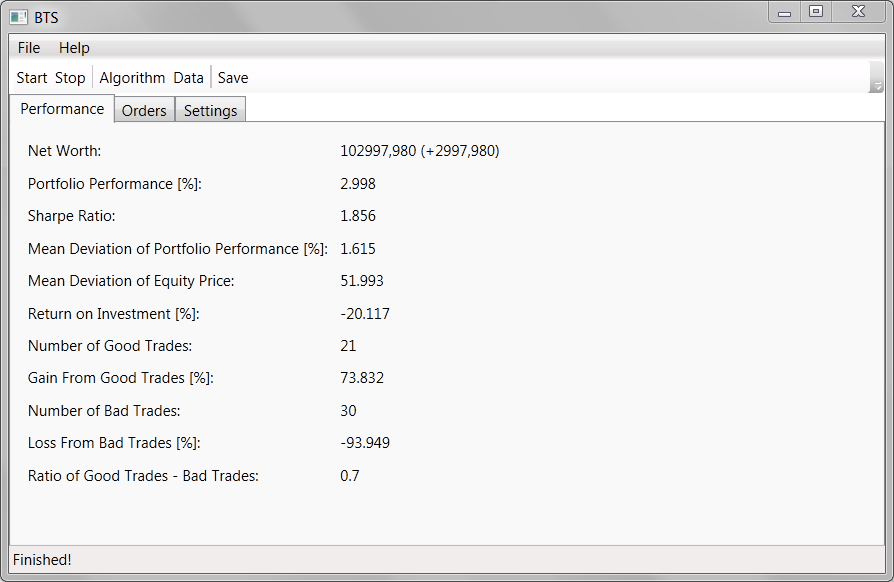
\includegraphics[width=1\textwidth]{images/btsperformance.png}
\caption{Start-Button der \gls{BTS}}
\end{figure}

Die meisten Informationen �ber den Verlauf des Tests k�nnen nun auf dem Orders-Tab gefunden werden. Hier wird zuerst oben ein Chart der Aktien-Preisdaten mit allen gew�hlten Indikatoren angezeigt. Durch Rechtsklick mit der Maus kann im Chart hinausgezoomt und mit der linken Maustaste hineingezoomt werden. Die Pfeile im Chart zeigen an, zu welchen Zeitpunkten der Algorithmus unter reellen Bedingungen �ber den gew�hlten Zeitabschnitt Signale ausgegeben h�tte. Die unterschiedlichen Farben und Farbschattierungen zeigen dabei ein Kauf- (Gr�n) oder ein Verkauf-Signal (Rot) und dessen St�rke an.\\
In der unteren H�lte des Bildschirms wird zu jedem dieser Signale ausgegeben welchen Effekt das jeweilige Signal auf das Kapital h�tte und welcher Gewinn oder Verlust dadurch zum damaligen Preis entstanden w�re. Position bzw. der Transaction Price geben dabei an, wieviele Round Lots durch dieses Signal gekauft worden w�ren und wieviel die Umsetzung des Signals kosten w�rde. Gain/Loss bezieht sich auf die prozentuelle Ver�nderung des Investitionskapitals der expliziten Order und Portfolio Performance auf die prozentuelle bzw. absolute Ver�nderung des gesamten gew�hlten Kapitals. All diese Werte werden auch kumulativ, also aufaddiert, angezeigt. 

\begin{figure}[H]
\centering
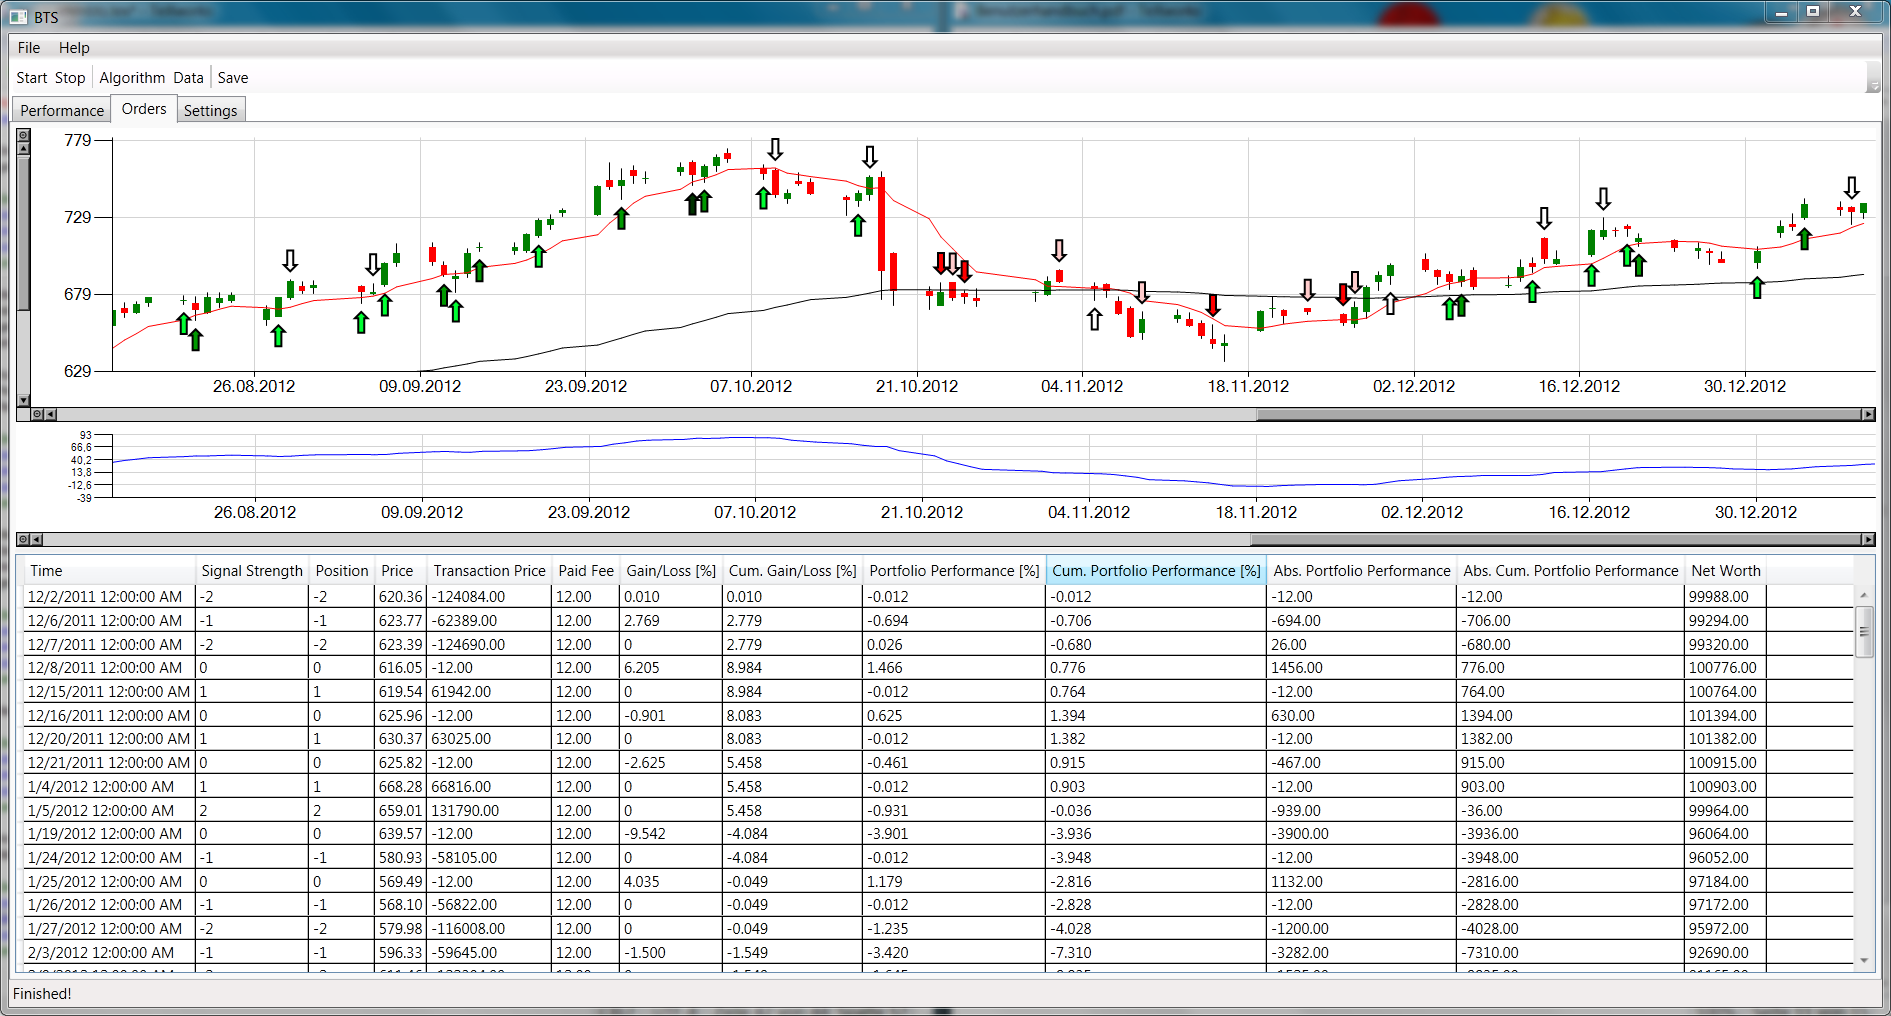
\includegraphics[width=1\textwidth]{images/btsorders.png}
\caption{Start-Button der \gls{BTS}}
\end{figure}

Zu guter Letzt k�nnen unter ''File'' -> ''Export'' die berechneten Performance-Daten lesbar als Text-File (.txt) exportiert werden. Au�erdem kann der aktuelle Zustand der \gls{BTS} inklusive aller Settings und berechneter Daten au�er der Charts (da sonst die Aktiendaten mitgespeichert werden m�ssten) gespeichert und zu einem sp�teren Zeitpunkt erneut geladen werden.
%!TEX root=../Benutzerhandbuch.tex
\chapter{Minimale Systemvoraussetzungen}
Folgende Vorraussetzungen m�ssen vom System erf�llt werden:\\
\textbf{Hardwareanforderungen}
\begin{center}
\begin{tabular}{ | l | c |}\hline 
Prozessor & 1 GHz \\ \hline
RAM & 512 MB \\ \hline
Festplattenspeicher (32 Bit) & 850 MB \\ \hline
Festplattenspeicher (64 Bit) & 2 GB \\ \hline
\end{tabular}
\end{center}
\textbf{Betriebssystemanforderungen} \\
Unterst�tzte Clientbetriebssysteme sind:
\begin{itemize}
\item Windows 8 (32-Bit- und 64-Bit-Editionen)
\item Windows 7 (32-Bit- und 64-Bit-Editionen)
\item Windows Vista (32-Bit- und 64-Bit-Editionen)
\end{itemize}

%\begin{landscape}

\chapter{Zeitaufzeichnungen}

\begin{figure}
	\centering
		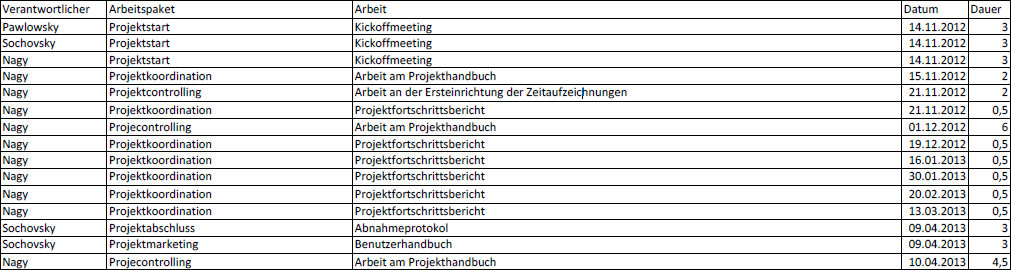
\includegraphics[width=1.2\textwidth, angle=90]{graphics/appendix/projektmanagement.PNG}
	\caption*{Projektmanagement}
\end{figure}

\begin{figure}
	\centering
		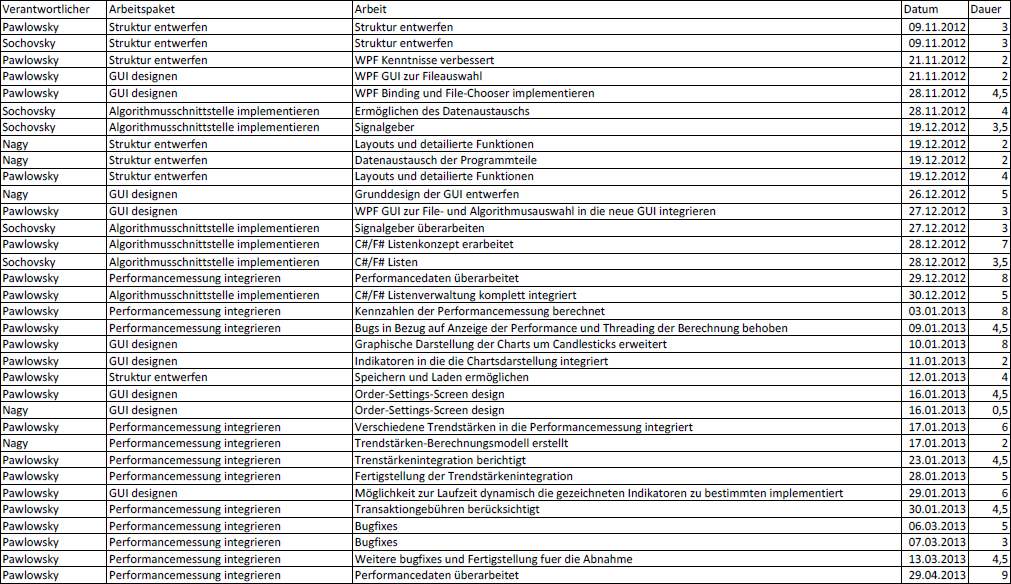
\includegraphics[width=1.2\textwidth, angle=90]{graphics/appendix/backtestingsoftware.PNG}
	\caption*{Backtesting-Software}
\end{figure}

\begin{figure}
	\centering
		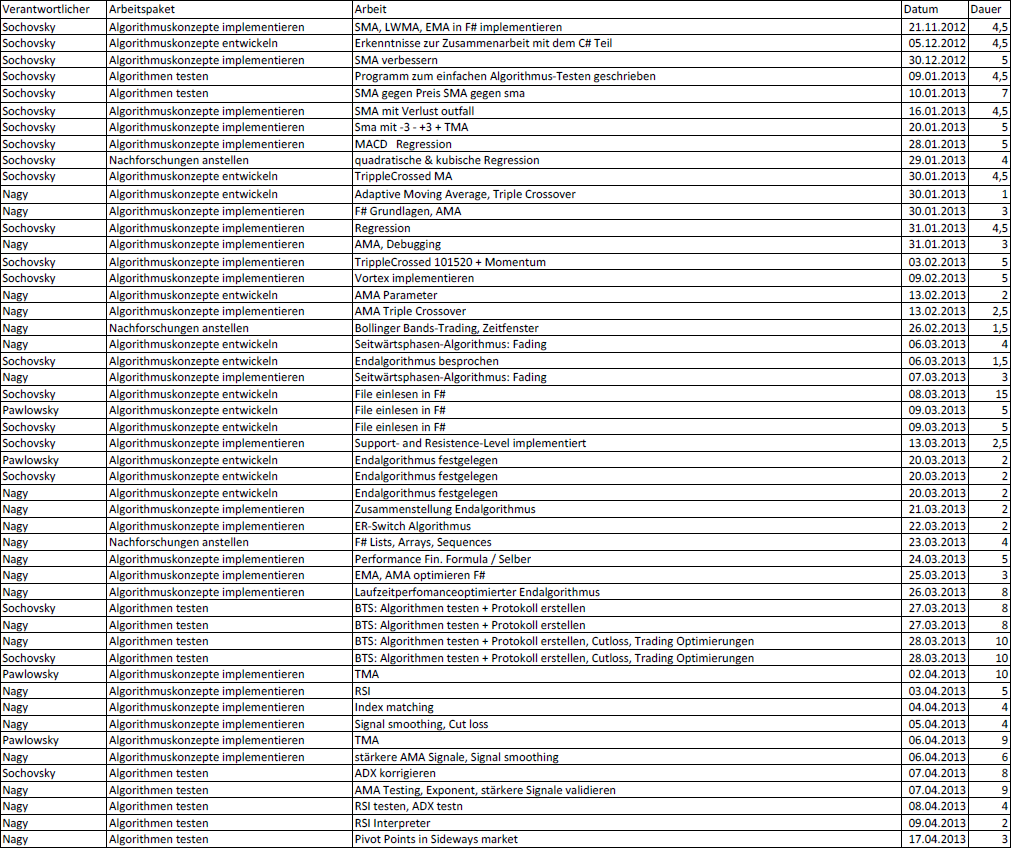
\includegraphics[width=1.2\textwidth, angle=90]{graphics/appendix/algorithmus.PNG}
	\caption*{Algorithmus}
\end{figure}

\begin{figure}
	\centering
		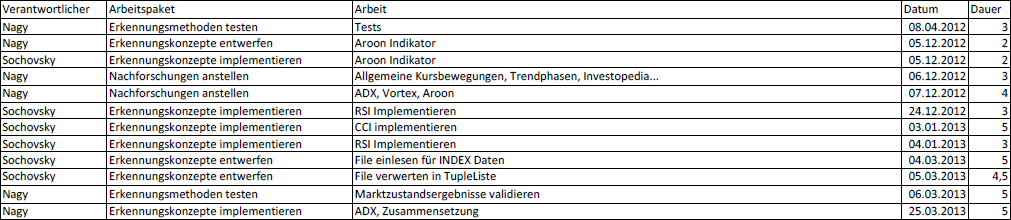
\includegraphics[width=1.2\textwidth, angle=90]{graphics/appendix/marktzustandserkennung.PNG}
	\caption*{Marktzustandserkennung}
\end{figure}

\begin{figure}
	\centering
		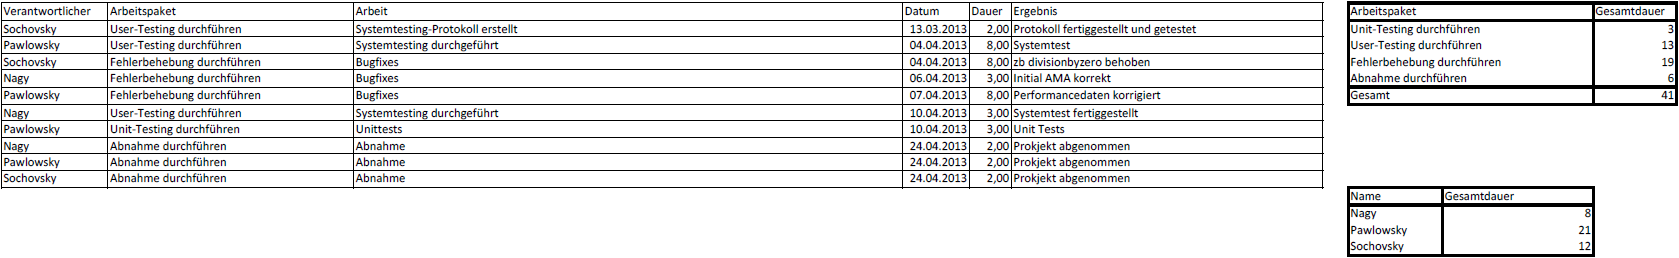
\includegraphics[width=1.2\textwidth, angle=90]{graphics/appendix/testingabschluss.PNG}
	\caption*{Testing \& Abschluss}
\end{figure}

%\end{landscape}